\documentclass[10pt,a4paper]{article}
\usepackage[utf8]{inputenc}
\usepackage[parfill]{parskip}
\usepackage[section]{placeins}
\usepackage{subfig}
\usepackage{graphicx}
\usepackage{array}
\usepackage{tabularx}
\usepackage[scientific-notation=true]{siunitx}
\usepackage{amsmath}
\usepackage{hyperref}
\usepackage{epigraph}

\author{Dominik Nerger (i6146759)}
\title{Text Mining South Park}
\date{\today}

\begin{document}
	\maketitle
	
	\tableofcontents
	\newpage
	\section{Introduction}
	\epigraph{ And tell everyone in the past for us, that no one single answer... is ever the answer. }{UAA Leader, Ep. Go God Go XII}

	South Park is an animated series revolving around the four boys Stan Marsh, Kyle Broflovski, Eric Cartman and Kenny McCormick who live in South Park, Colorado. South Park has the third most episodes in regard to American animated TV series, totaling 277 episodes over 20 seasons. 
	
	Because of the huge amount of episodes, it is an interesting target for the practical assignment, which is part of the course \textit{Information Retrieval \& Text Mining}, with the possibility of acquiring new insights into a TV series that is used to satirize American culture. 
	
	
	
	The repository is available on GitHub\footnote{\url{https://github.com/dnerger/South-Park-Text-Mining}}.
	\section{Libraries}
	
	All scripts have been programmed in \textit{R}. To execute the scripts, R needs to be installed. To view temporary files that are executed during runtime, e.g. the corpus or a TermDocumentMatrix, it is advised to install RStudio. The libraries necessary for each script are imported at the top of each script, if they are not installed they can be installed by executing:
	
	\begin{verbatim}
	install.packages("library-name")
	\end{verbatim}
	
	In the following, all libraries that are related to Text Mining techniques will be introduced shortly.
	
	The library \textbf{tm} is the Text Mining package of R, which enables pre-processing of data sets and allows to build the corpus. \textbf{RWeka} is a collection of machine learning algorithms for data mining tasks. \textbf{NMF} introduces the Non-negative Matrix Factorization to R.
	\textbf{NLP} and \textbf{OpenNLP} are libraries that provide Natural Language Processing techniques and are used for NER-Tagging. \textbf{syuzhet} extracts sentiments from text and contains the three sentiment dictionaries \textit{bing}, \textit{afinn} and \textit{nrc}.
	The package \textbf{stm} is used for Structural Topic Modeling  which is LDA with additional met-data and can be visualized using the package \textbf{LDAvis}.
	Libraries used for visualization include \textbf{igraph},\textbf{ggplot2}, \textbf{ggraph}, \textbf{viridis} and \textbf{wordcloud}.
	
	\section{Data set}	
	The data set spans from seasons \textbf{1} to \textbf{18}, adding up to 257 episodes overall with a file size of 5.41MB. It contains 70896 rows, with each row possessing information about the \textbf{season}, \textbf{episode}, \textbf{character} and \textbf{line} and is available as a \textit{.csv} file.
	
	The data set has been crawled by Bob Adams and is available to download on GitHub\footnote{\url{https://github.com/BobAdamsEE/SouthParkData}}. It has been assembled by crawling the South Park Archives\footnote{\url{http://southpark.wikia.com/wiki/South_Park_Archives}}. The code of this GitHub repository is not available to the public.
	
	 I made an attempt at a crawl with the R package \textbf{rvest}, which is able to harvest data from websites.  However, the \textit{html data} of the episode scripts provided on the South Park Archives differ between episodes. For 16 of 20 seasons, the whole episode needs to be pre-processed manually because the \textbf{line} and \textit{character} are extracted individually and can not be merged because of random whitespace lines that are introduced by \textbf{rvest}.
	 
	 The data set is used in three different versions:
	 \begin{enumerate}
	 \item \textit{dialogue} - each entry holds information about season, episode, character and line
	 \item \textit{by.season} - each entry holds information about season and the complete script for that season
	 \item \textit{by.episode} - each entry holds information about that episode, season and script for that episode
	 \end{enumerate}
	 
	 Both \textit{by.episode} and \textit{by.season} are created by using the data from \textit{dialogue}.
	
	
	\begin{figure}[h]
	\centering
	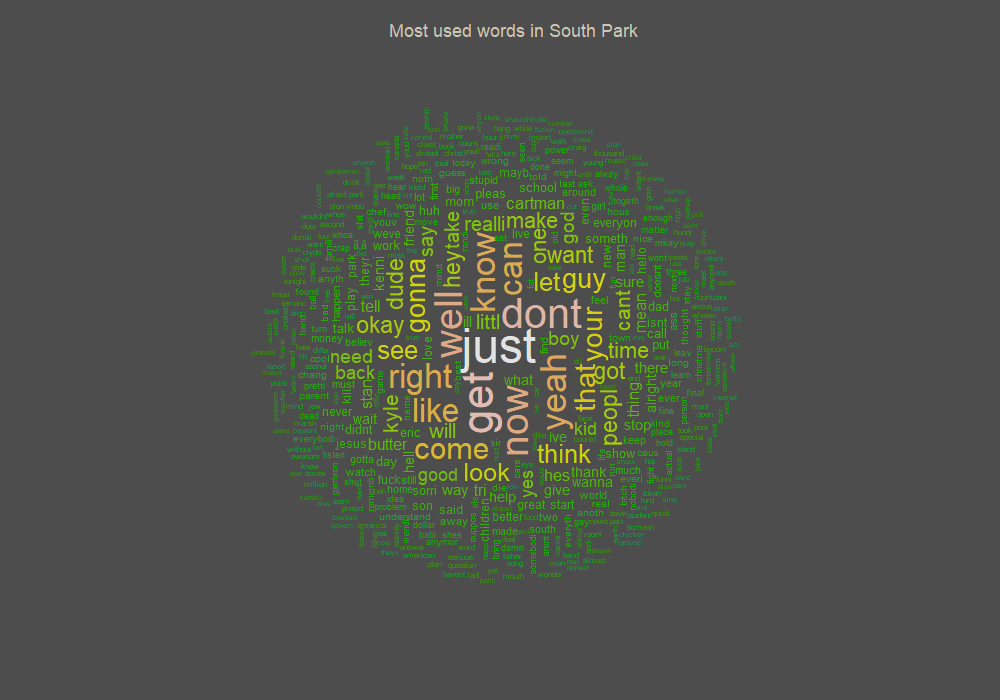
\includegraphics[scale=0.9]{images/WordCloud.png}
	\caption{General wordcloud, containing terms by frequency}
	\label{fig:WordCloud}
	\end{figure}
	
	\begin{figure}[h]
	\centering
	\includegraphics[scale=0.9]{images/WordCloud-TFIDF.png}
	\caption{Wordcloud containing terms by TF-IDF score}
	\label{fig:WordCloud-TFIDF}
	\end{figure}
	\begin{figure}[h]
	\centering
	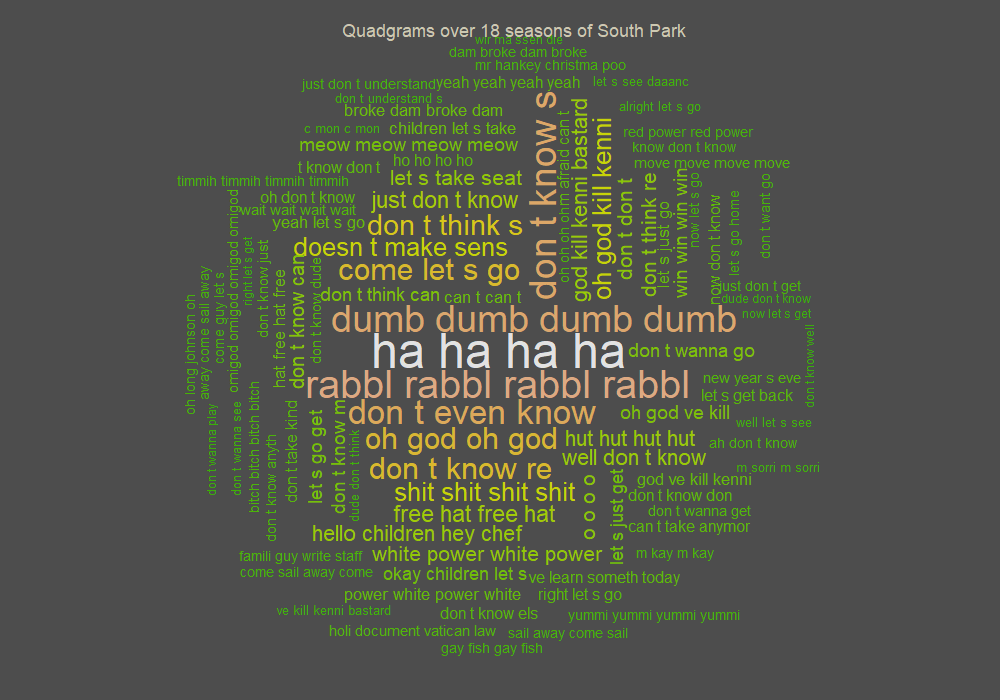
\includegraphics[scale=0.9]{images/WordCloud-ngram.png}
	\caption{Wordcloud containing ngrams (n=4) by frequency}
	\label{fig:WordCloud-ngram}
	\end{figure}
	
	\begin{figure}[h]
	\centering
	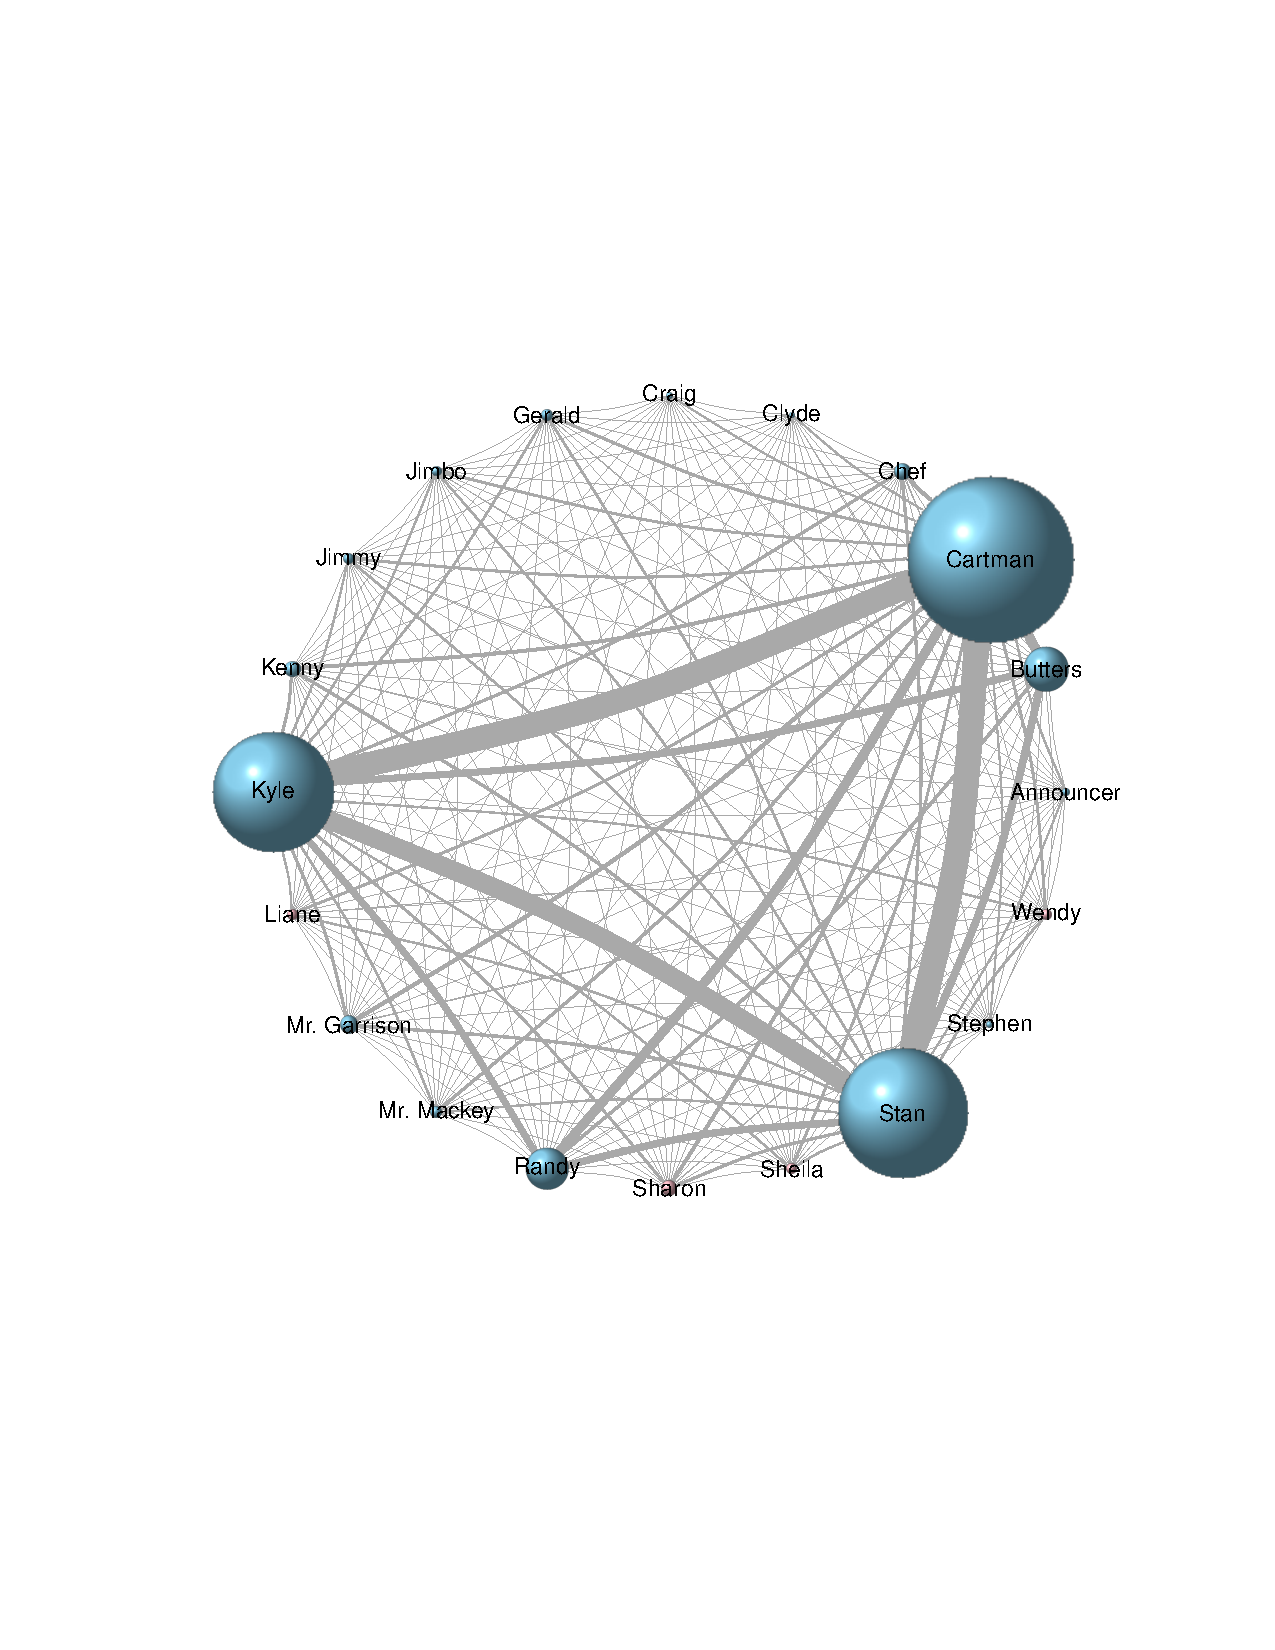
\includegraphics[scale=0.7]{images/CoOccurence Matrix.pdf}
	\caption{Co-occurences of characters over 257 episodes, size of vertex in relation to amount of lines}
	\label{fig:CoOccurence}
	\end{figure}
	
	
	\section{Pre-processing}
	In general, the standard pre-processing tasks are executed on the corpus. Depending on the later use, different packages perform these.
	The package \textbf{tm} is used to convert the corpus to lower case, remove punctuation and numbers as well as strip whitespaces. Furthermore, stopwords are removed using the stopword list from the Snowball stemmer project  the corpus is stemmed using Porter's stemming algorithm.\footnote{\url{http://snowball.tartarus.org/algorithms/english/stop.txt}} It is used together with several DocumentTerm- and TermDocument-Matrices.
	
	The pre-processing for the Structural Topic Model is done with the same tasks, however those are performed by the package \textbf{stm} itself.
	
	For the Named Entity Recognition with package \textbf{openNLP}, no pre-processing tasks are performed. They can be executed and might improve the overall runtime, but it does not change the overall result. Especially stemming and the lower case convertion could decrease the results because stemmed or lower case entities, as well as the sentiments that are mined, will not be recognized.

	
	
	\section{Results and visualization}
	
	
	\section{Conclusion}
	In conclusion, 

	\section{Future work}
\end{document}
